%%%%%%%%%%%%%%%%%%%%%%%%%%%%%%%%%%%%%%%%%%  不使用 authblk 包制作标题  %%%%%%%%%%%%%%%%%%%%%%%%%%%%%%%%%%%%%%%%%%%%%%
%-------------------------------PPT Title-------------------------------------
\title{03-密度泛函理论}
%-----------------------------------------------------------------------------

%----------------------------Author & Date------------------------------------
%\author[\textrm{Jun\_Jiang}]{姜\;\;骏\inst{}} %[]{} (optional, use only with lots of authors)
%% - Give the names in the same order as the appear in the paper.
%% - Use the \inst{?} command only if the authors have different
%%   affiliation.
\institute[BCC]{\inst{}%
%\institute[Gain~Strong]{\inst{}%
\vskip -20pt 北京市计算中心}
%\vskip -20pt {\large 格致斯创~科技}}
\date[\today] % (optional, should be abbreviation of conference name)
{%	{\fontsize{6.2pt}{4.2pt}\selectfont{\textcolor{blue}{E-mail:~}\url{jiangjun@bcc.ac.cn}}}
\vskip 45 pt {\fontsize{8.2pt}{6.2pt}\selectfont{%清华大学\;\;物理系% 报告地点
	\vskip 5 pt \textrm{2022.07.08}}}
}

%% - Either use conference name or its abbreviation
%% - Not really information to the audience, more for people (including
%%   yourself) who are reading the slides onlin%%   yourself) who are reading the slides onlin%%   yourself) who are reading the slides onlineee
%%%%%%%%%%%%%%%%%%%%%%%%%%%%%%%%%%%%%%%%%%%%%%%%%%%%%%%%%%%%%%%%%%%%%%%%%%%%%%%%%%%%%%%%%%%%%%%%%%%%%%%%%%%%%%%%%%%%%

\subject{}
% This is only inserted into the PDF information catalog. Can be left
% out.
%\maketitle
\frame
{
%	\frametitle{\fontsize{9.5pt}{5.2pt}\selectfont{\textcolor{orange}{“高通量并发式材料计算算法与软件”年度检查}}}
\titlepage
}
%-----------------------------------------------------------------------------

%------------------------------------------------------------------------------列出全文 outline ---------------------------------------------------------------------------------
%\section*{}
%\frame[allowframebreaks]
%{
%  \frametitle{Outline}
%%  \frametitle{\textcolor{mycolor}{\secname}}
%  \tableofcontents%[current,currentsection,currentsubsection]
%}
%%在每个section之前列出全部Outline
%%类似的在每个subsection之前列出全部Outline是\AtBeginSubsection[]
%\AtBeginSection[]
%{
%  \frame<handout:0>%[allowframebreaks]
%  {
%    \frametitle{Outline}
%%全部Outline中,本部分加亮
%    \tableofcontents[current,currentsection]
%  }
%}

%-----------------------------------------------PPT main Body------------------------------------------------------------------------------------
\small
\section{密度泛函理论}       %Bookmark
\subsection{\rm{Thomas-Fermi~}模型}       %Bookmark
\frame
{
	\frametitle{\textrm{Thomas-Fermi}模型} 
	1927年,\textrm{Thomas}和\textrm{Fermi}基于均匀电子气模型上建立\textrm{Thomas-Fermi}模型,\textcolor{blue}{体系能量可用}\textcolor{red}{电子密度}\textcolor{blue}{表示}:
	\begin{itemize}
		\item 动能表达式
			$$T_{\mathrm{TF}}[\rho(\vec r)]=\dfrac3{10}(3\pi^2)^{\frac23}\int\rho^{\frac53}(\vec r)\mathrm{d}\vec r$$
		\item 外势$V_{ext}(\vec r)$下电子体系的能量泛函表达式为
			\begin{displaymath}
				\begin{aligned}
					E_{\mathrm{TF}}[\rho(\vec r)]=&\dfrac3{10}(3\pi^2)^{\frac23}\int\rho^{\frac53}(\vec r)\mathrm{d}\vec r\\
					&+\int\rho(\vec r)V_{ext}(\vec r)\mathrm{d}\vec r+\dfrac12\int\int\dfrac{\rho(\vec r_1)\rho(\vec r_2)}{|\vec r_2-\vec r_1|}\mathrm{d}\vec r_1\mathrm{d}\vec r_2
				\end{aligned}
			\end{displaymath}
		\item \textrm{Thomas-Fermi}模型完全没有考虑电子的交换-相关作用
	\end{itemize}
}

\frame
{
	\frametitle{\textrm{Thomas-Fermi-Dirac}模型} 
	1930年,\textrm{Dirac}将\textrm{Thomas-Fermi}模型修正,用局域密度近似考虑电子交换作用
			\begin{displaymath}
				\begin{aligned}
					E_{\mathrm{TFD}}[\rho(\vec r)]=&\dfrac3{10}(3\pi^2)^{\frac23}\int\rho^{\frac53}(\vec r)\mathrm{d}\vec r+\int\rho(\vec r)V_{ext}(\vec r)\mathrm{d}\vec r\\
					&+\dfrac12\int\int\dfrac{\rho(\vec r_1)\rho(\vec r_2)}{|\vec r_2-\vec r_1|}\mathrm{d}\vec r_1\mathrm{d}\vec r_2-\dfrac34\bigg(\dfrac3{\pi}\bigg)^{\frac13}\int\rho^{\frac43}(\vec r)\mathrm{d}\vec r
				\end{aligned}
			\end{displaymath}
			\begin{itemize}
				\item 在总电子数守恒约束条件
					$$\int\rho(\vec r)\mathrm{d}\vec r=N$$
					下,能量泛函$E_{\mathrm{TFD}}[\rho(\vec r)]$对密度$\rho(\vec r)$的变分极小获得体系的基态密度和基态能量
			\end{itemize}
}

\frame
{
	\frametitle{\textrm{Thomas-Fermi}模型}
	\begin{itemize}
		\item \textrm{Thomas-Fermi}模型用电子密度代替波函数描述问题是极大的简化,但模型过于粗糙:\\
%			\begin{enumerate}
%				\item 以均匀电子气的密度得到动能的表达式
%				\item 完全忽略电子间的交换-相关作用
%			\end{enumerate}
			不能正确描述相互作用电子体系的基本特征,如原子的壳层结构
		\item \textrm{Thomas-Fermi}模型虽不够精确,但可以通过引入修正项校正:
			\textrm{Dirac}交换泛函 $$E_X[\rho(\vec r)]=-\dfrac34\bigg(\dfrac3{\pi}\bigg)^{\frac13}\int\rho^{\frac43}(\vec r)\mathrm{d}\vec r$$
			\textrm{Wigner}相关泛函 $$E_C[\rho(\vec r)]=-0.056\int\dfrac{\rho^{\frac43}(\vec r)}{0.079+\rho^{\frac13}(\vec r)}\mathrm{d}\vec r$$
	\end{itemize}
	\textrm{Thomas-Fermi}模型为密度泛函理论\textrm{(DFT)}提供了重要的启示
}

\subsection{密度泛函理论}       %Bookmark
\frame                               %
{
\frametitle{密度泛函理论(\textrm{DFT})} %Slide Page Title
%   \secname
与传统的量子力学方法不同,密度泛函理论的基本变量是体系的基态电子密度。%通过体系的电子密度而非波函数确定体系的基态能量。
\begin{itemize}%[+-| alert@+>]
	\item 密度泛函理论的基石:\textrm{Hohenberg-Kohn}定理\upcite{PR136-B864_1964}
\vskip 5pt
\begin{itemize}%[+-| alert@+>]
   \setlength{\itemsep}{8pt}
 \item $E[\rho]=F_{\mathrm{HK}}[\rho]+\displaystyle\int\rho(\vec{r})v(\vec{r})\textrm{d}\vec{r}$ \\
\vskip 5pt 其中$F_{\mathrm{HK}}[\rho]=\underset{\Psi\to\rho}{\mathrm{Min}}\langle\Psi[\rho]|\hat{T}+\hat{W}|\Psi[\rho]\rangle$
是普适的泛函表达式。%,指明多电子体系的基态性质与基态密度间存在一一对应关系
     \textrm{\small{第一定理表明多电子体系的性质完全由体系的基态密度决定}}
   \item 如果$\tilde\Psi\neq\Psi$,
     $E[\tilde\rho]\geqslant E[\rho_0]$\\
     \textrm{\small{第二定理指出基态总能量泛函在体系基态电子密度处取极小值}}
   \end{itemize}
%\textrm{\small{第二定理指出基态总能量泛函在体系基态电子密度处取极小值}}
\vskip 8pt
 \item 密度泛函理论的优越性:用密度($\rho$)代替波函数($\Psi$)描述体系
\vskip 5pt
 \item 密度泛函理论的困难:能量密度泛函的精确形式未知
   \end{itemize}
}

\frame                               %
{
\frametitle{密度泛函理论(\textrm{DFT})}
\textrm{Kohn-Sham}方程\upcite{PR140-A1133_1965}:无相互作用体系+交换-相关能的贡献
$$(T_S+V_{e\!f\!f})|\varphi_i\rangle=\varepsilon_i|\varphi_i\rangle,\quad i=1,\cdots,N,\cdots$$
其中$T_S=-\dfrac12\nabla^2$~~是无相互作用体系的动能
\begin{displaymath}
	\begin{aligned}
		V_{e\!f\!f}(\vec r)=&V_{ext}(\vec r)+\displaystyle\int w(\vec r,\vec r\,')\rho(\vec r\,')\mathrm{d}\vec r\,'+V_{\mathrm{XC}}[\rho]\\
=&\displaystyle\int\dfrac{\rho(\vec r\,')}{|\vec r-\vec r^{\prime}|}\mathrm{d}\vec r\,'+V_{ext}(\vec r)+V_{\mathrm{XC}}[\rho]
	\end{aligned}
\end{displaymath}
$V_{ext}(\vec r)$是电子体系与外部的电荷或磁场相互作用\\
$V_{\mathrm{XC}}[\rho]=\dfrac{\delta E_{\mathrm{XC}}}{\delta\rho(\vec r)}$称为交换-相关势
\vskip 10pt
\textrm{Kohn-Sham}方程是形式上的单粒子方程
\vskip 6pt
\textrm{Kohn-Sham}方程的实质:\\\textcolor{red}{将动能泛函的主要部分分离出来,剩余部分放在交换-相关能中}
}

\frame
{
\frametitle{交换-相关能与交换-相关势}
实际考虑交换-相关能时,会将交换-相关能表示为交换能和相关能之和:
\begin{displaymath}
	E_{\mathrm{XC}}[\rho]=E_{\mathrm{X}}[\rho]+E_{\mathrm{C}}[\rho]=\int\varepsilon_{\mathrm{X}}[\rho]\rho(\vec{r}) \textrm{d}^3\vec{r}+\int\varepsilon_{\mathrm{C}}[\rho]\rho(\vec{r}) \textrm{d}^3\vec{r}
\end{displaymath}
$\varepsilon_{\mathrm{X}}[\rho]$和$\varepsilon_{\mathrm{C}}[\rho]$可理解为单电子的交换能和相关能
\vskip 20pt
交换-相关势通过交换-相关能计算得到:~
		\begin{displaymath}
			V_{\mathrm{XC}}^{\sigma}[\rho_{\alpha},\rho_{\beta}]=\dfrac{\delta E_{\mathrm{XC}}[\rho_{\alpha},\rho_{\beta}]}{\delta\rho_{\sigma}}=\dfrac{\delta\{E_{\mathrm{X}}[\rho_{\alpha},\rho_{\beta}]+E_{\mathrm{C}}[\rho_{\alpha},\rho_{\beta}]\}}{\delta\rho_{\sigma}}
		\end{displaymath}
		\textcolor{red}{注意}:~由于$E_{\mathrm{XC}}[\rho_{\sigma}]$对$\rho_{\sigma}$是非线性的\\
		\textcolor{blue}{$V_{\mathrm{XC}}=V_{\mathrm{X}}+V_{\mathrm{C}}$和$\varepsilon_{\mathrm{XC}}=\varepsilon_{\mathrm{X}}+\varepsilon_{\mathrm{C}}$不同,不要混淆这两个量}
}
%  \beamertemplateshadingbackground{blue!10}{yellow!10}

\frame                               %
{
\frametitle{交换-相关能密度泛函}
\textcolor{blue}{密度泛函理论的核心问题}:\\
\textrm{Kohn-Sham}方程用于实际计算,必须知道$E_{XC}[\rho]$或者$V_{XC}[\rho]$与$\rho(\vec r)$的泛函关系
\vskip 15pt
\begin{minipage}[b]{0.59\textwidth}
 \hspace*{-15pt}
 {\fontsize{7.5pt}{6.0pt}\selectfont\begin{itemize}%[+-| alert@+>]
	 \setlength{\itemsep}{10pt}
 \item \textrm{LDA}:泛函只与密度分布的局域值有关
 \item \textrm{GGA}:泛函依赖:局域密度及其梯度
 \item $meta$-\textrm{GGA}:泛函依赖的变量还有动能密度
 \item 杂化(\textrm{hybrid})泛函:泛函与占据轨道有关
 \item 其他的交换-相关能泛函
 \item<1-> 完全非局域泛函:理想泛函,不现实
 \end{itemize}}
\end{minipage}
\hfill
\begin{minipage}[b]{0.39\textwidth}
\hspace*{-10pt}
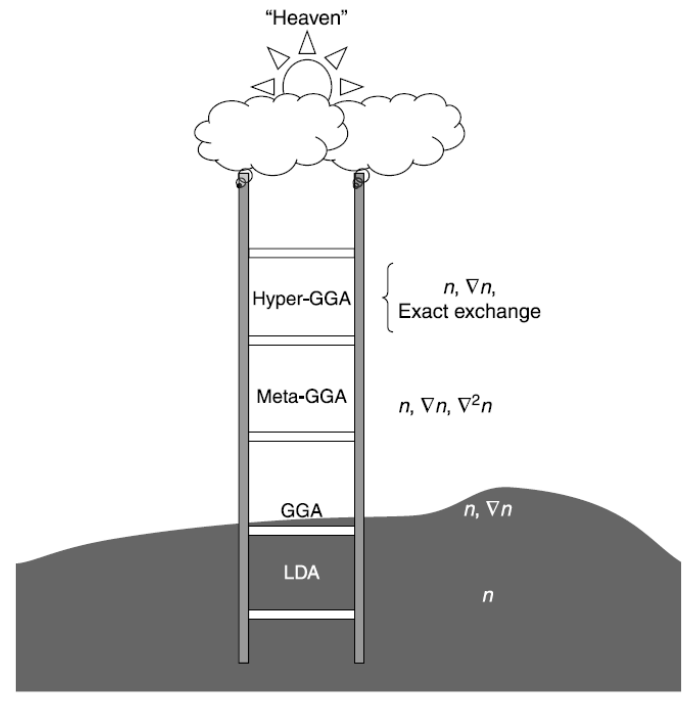
\includegraphics[height=1.7in,width=3.18in,viewport=10 5 1380 700,clip]{Figures/Jacobi-ladder.png}\\
\centering{\textcolor{red}{\textrm{\tiny Jacob's ladder}}}
\end{minipage}
% \begin{itemize}%[+-| alert@+>]
%\item 交换-相关能密度泛函
}

\frame                               %
{
	\frametitle{近似能量泛函$E_{\mathrm{XC}}[\rho]$的主要问题}
\vskip 20pt
\begin{enumerate}%[+-| alert@+>]
   \setlength{\itemsep}{10pt}
 \item  密度是整体变量:~电子自相互作用抵消不净\\%\quad\textrm{(LDA+U)}方法的校正%(\textrm{LDA+U})
	 用\textrm{DFT}计算电子数很少的体系,一般都会有较大的误差
 \item  电子相关:~简并和近简并基态的表示不合理\\
	 基态电子密度用不同的简并轨道计算时,体系能量应保持不变,但现有的近似能量泛函不具有这个性质
 \item  渐近行为:~处理弱相互作用体系的误差大\\
	 如\textrm{Van der Waals}相互作用和现有近似能量泛函本身的计算误差在同一量级
 \end{enumerate}
}

\frame                               %
{
	\frametitle{\textrm{Kohn-Sham}方程}
\begin{figure}[h!]
\centering
\vspace*{-0.21in}
\hspace*{-0.1in}
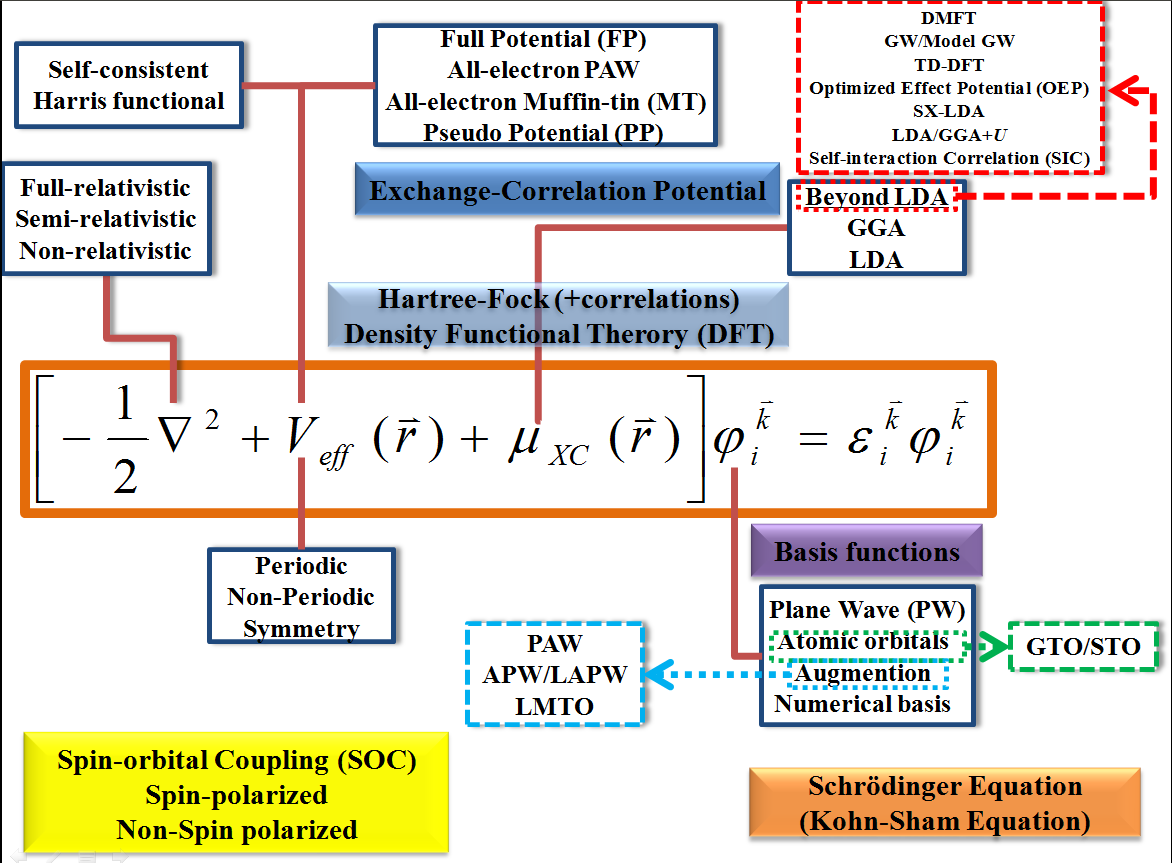
\includegraphics[height=2.7in,width=4.0in,viewport=2 5 1162 880,clip]{Figures/DFT.png}
\caption{\tiny \textrm{The Analysis of Kohn-Sham equation.}}%(与文献\cite{EPJB33-47_2003}图1对比)
\label{DFT}
\end{figure}
}

\frame
{
	\frametitle{\textrm{DFT-SCF}}
\begin{figure}[h!]
\centering
\vspace*{-0.25in}
\hspace*{-0.80in}
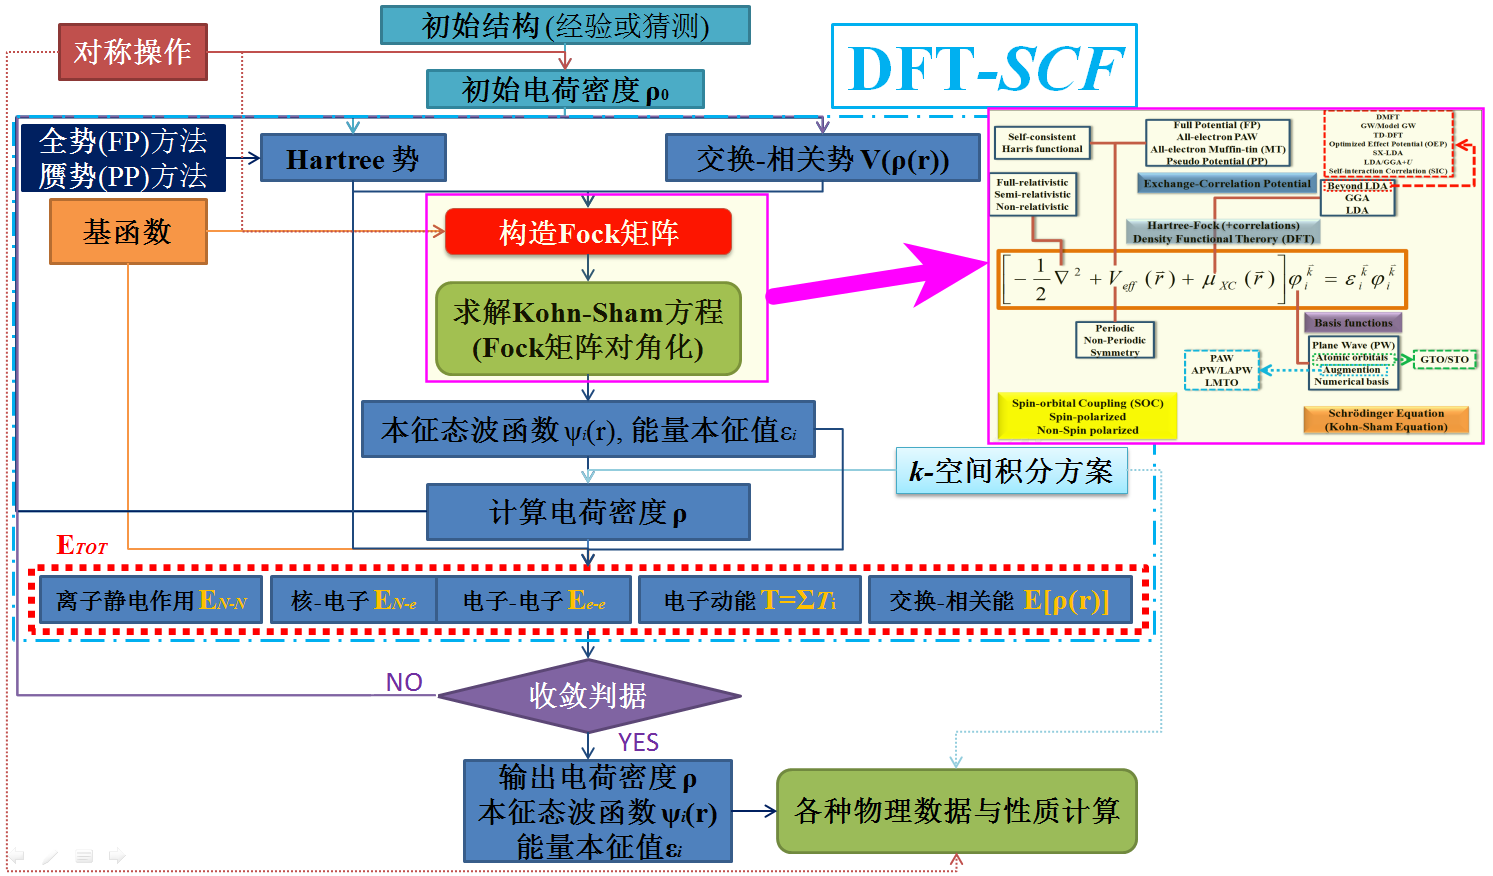
\includegraphics[height=2.80in,width=4.95in,viewport=5 3 1490 870,clip]{Figures/DFT-SCF_2.png}
%\caption{\tiny \textrm{Pseudopotential for metallic sodium, based on the empty core model and screened by the Thomas-Fermi dielectric function.}}%(与文献\cite{EPJB33-47_2003}图1对比)
\label{DFT-SCF-2}
\end{figure}
}

\subsection{常见泛函的一些形式}
\frame%[allowframebreaks]
{
	\frametitle{\rm{LDA}泛函}
	\begin{itemize}
		\item 交换能部分
	\begin{displaymath}
		\begin{aligned}
			\varepsilon_{\mathrm{X}}[\rho,\zeta]=&2^{-1/3}C_{\mathrm{X}}^{\sigma}g(\zeta)\rho^{1/3}(\vec r)\\
			E_{\mathrm{X}}[\rho,\zeta]=&\int\varepsilon_{\mathrm{X}}[\rho,\zeta]\rho(\vec r)\mathrm{d}\vec r\\
		\end{aligned}
	\end{displaymath}
	{\fontsize{7.5pt}{6.0pt}\selectfont{这里:~$C_{\mathrm{X}}^{\sigma}=\dfrac32\bigg(\dfrac3{4\pi}\bigg)^{1/3}$\\
		$g(\zeta)=\dfrac12\bigg[(1+\zeta)^{4/3}+(1-\zeta)^{4/3}\bigg]$\\
		$\zeta(\vec r)=\dfrac{[\rho_{\alpha}(\vec r)-\rho_{\beta}(\vec r)]}{[\rho_{\alpha}(\vec r)+\rho_{\beta}(\vec r)]}$}}
	\end{itemize}
}

\frame%[allowframebreaks]
{
	\frametitle{\rm{LDA}泛函}
	\begin{itemize}
		\item 相关能部分
			\begin{displaymath}
				\hspace*{-30pt}	\varepsilon_{\mathrm{C}}^{\mathrm{LDA}}(r_s,\zeta)=\varepsilon_{\mathrm{C}}(r_s,0)+a_{\mathrm{c}}(r_s)\dfrac{f(\zeta)}{f^{\prime\prime}(\zeta)}(1-\zeta^4)+[\varepsilon_{\mathrm{c}}(r_s,1)-\varepsilon_{\mathrm{c}}(r_s,0)]f(\zeta)\zeta^4
			\end{displaymath}
			{\fontsize{7.5pt}{6.0pt}\selectfont{这里:~$r_s=\bigg[\dfrac3{4\pi}(\rho_{\alpha}+\rho_{\beta})^{-1}\bigg]^{1/3}$~$f(\zeta)=[(1+\zeta)^{4/3}+(1-\zeta)^{4/3}-2]/(2^{4/3}-2)$\\
			$\varepsilon_{\mathrm{C}(r_s,0)}$、$\varepsilon_{\mathrm{C}(r_s,1)}$、$a_{\mathrm{C}(r_s)}$由经验公式
			\begin{displaymath}
				\begin{aligned}
					&G(r_s,A,\alpha_1,\beta_1,\beta_2+\beta_3+\beta_4)\\
					=&-2A(1+\alpha_1r_s)\ln\bigg[1+\dfrac1{2A(\beta_1r_s^{1/2}+\beta_2r_s+\beta_2r_s^{3/2}+\beta_1r_s^2)}\bigg]
				\end{aligned}
			\end{displaymath}
		计算。其中$A$、$\alpha_1$、$\beta_1$、$\beta_2$、$\beta_3$、$\beta_4$是参数,通过拟合实验结果确定}}
		\begin{displaymath}
			E_{\mathrm{C}}[\rho]=\int\rho(\vec r)\varepsilon_{\mathrm{C}}(\vec r)\mathrm{d}\vec r
		\end{displaymath}
	\end{itemize}
}

\frame%[allowframebreaks]
{
	\frametitle{\rm{GGA}泛函}
	\begin{itemize}
		\item 交换能泛函:
			\begin{itemize}
				\item \textrm{PW91}
					\begin{displaymath}
						\begin{aligned}
							E_{\mathrm{X}}^{\mathrm{PW91}}[\rho_{\alpha},\rho_{\beta}]=&\dfrac12(E_{\mathrm{X}}^{\mathrm{PW91}}[2\rho_{\alpha}]+E_{\mathrm{X}}^{\mathrm{PW91}}[2\rho_{\beta}])\\
							E_{\mathrm{X}}^{\mathrm{PW91}}[\rho]=&-\dfrac34\bigg(\dfrac3\pi\bigg)^{1/3}\int\rho^{4/3}(\vec r)F(x)\mathrm{d}\vec r
						\end{aligned}
					\end{displaymath}
					\hspace*{-30 pt}{\fontsize{4.5pt}{4.0pt}\selectfont{这里:~$F(x)=\dfrac{1+0.19645(hx)\sinh^{-1}(7.7956hx)+(hx)^2\{0.2743-0.1508\mathrm{exp}[-100(hx)^2]\}}{1+0.19645(hx)\sinh^{-1}(7.7956hx)+0.004(hx)^4}$}\\
					$h=(24\pi^2)^{-1/3}$,~~~$x=|\nabla\rho|\rho^{-4/3}$}
				\item \textrm{PBE}
			\begin{displaymath}
				E_{\mathrm{X}}^{\mathrm{PBE}}[\rho,x]=E_{\mathrm{X}}^{\mathrm{LDA}}[\rho,x]-C_{\mathrm{X}}\int a\bigg(1-\dfrac1{bx^2}\bigg)\rho^{4/3}(\vec r)\mathrm{d}\vec r
			\end{displaymath}
			{\fontsize{4.5pt}{4.0pt}\selectfont{其中:~$C_{\mathrm{X}}=\dfrac34\bigg(\dfrac3\pi\bigg)^{1/3}$\\$a=0.804$,~~~$b=0.273$~是非经验参数}}
			\end{itemize}
	\end{itemize}
}

\frame%[allowframebreaks]
{
	\frametitle{\rm{GGA}泛函}
	\begin{itemize}
		\item 相关能泛函:
			\begin{itemize}
				\item \textrm{PW91}
					\begin{displaymath}
						\begin{aligned}
							E_{\mathrm{C}}^{\mathrm{PW91}}[\rho_{\alpha},\rho_{\beta}]=&\int\mathrm{d}\vec r\rho(\vec r)[\varepsilon_{\mathrm{C}}^{\mathrm{LSDA}}(r_s,\zeta)]+H(t,r_s,zeta)\\
							H=&H_0+H_1
						\end{aligned}
					\end{displaymath}
					{\fontsize{4.5pt}{4.0pt}\selectfont{这里:~
						\begin{displaymath}
							\begin{aligned}
								H_0=&f^3(\zeta)\dfrac{\beta^2}{2\alpha}\ln\bigg(1+\dfrac{2\alpha}{\beta}\dfrac{t^2+At^4}{1+At^2+A^2t^4}\bigg)\\
								A=&\dfrac{2\alpha}{\beta}\dfrac1{\mathrm{exp[-2\alpha\varepsilon_{\mathrm{C}}^{\mathrm{LDA}}(r_s,\zeta)}/f^3(\zeta)\beta^2]-1}\\
							t=&\dfrac{|\nabla\rho|}{2f(\zeta)k_s\rho}~~~f(\zeta)=\dfrac12\bigg[(1+\zeta)^{2/3}+(1-\zeta)^{2/3}\bigg]\\
							k_s=&[4(3\pi^{-1}\rho)^{1/3}]^{1/2}
							\end{aligned}
						\end{displaymath}
						参数 $\alpha=0.09$,~~~$\beta=\nu C_{\mathrm{C}}(0)$\\
						$\nu=(16/\pi)(3\pi^2)^{1/3}$,~~~$C_{\mathrm{C}}(0)=0.004235$
				}}
			\end{itemize}
	\end{itemize}
}

\frame%[allowframebreaks]
{
	\frametitle{\rm{meta-GGA}泛函}
	\begin{itemize}
		\item 交换能泛函
			\begin{itemize}
				\item \textrm{TPSS}
					\begin{displaymath}
						\begin{aligned}
							E_{\mathrm{X}}^{\mathrm{TPSS}}[\rho]&=\int\mathrm{d}\vec r\rho(\vec r)\varepsilon_{\mathrm{X}}^{\mathrm{LSDA}}(\vec r)F_{\mathrm{X}}^{\mathrm{LSDA}}(p,z)\\
							F_{\mathrm{X}}^{\mathrm{TPSS}}&=1+\kappa-\dfrac{\kappa}{1+x/\kappa}
						\end{aligned}
					\end{displaymath}
{\fontsize{4.5pt}{4.0pt}\selectfont{这里:~
	$\rho(\vec r)=\rho_{\alpha}(\vec r)+\rho_{\beta}({\vec r})$,~~~$\varepsilon_{\mathrm{X}}^{\mathrm{LSDA}}(\vec r)=-\dfrac3{4\pi}[3\pi^2\rho(\vec r)]^{1/3}$
\\
\begin{displaymath}
	\begin{aligned}
		x=&\left\{\bigg[\dfrac{10}{81}+\dfrac{cz^2}{(1+z^2)^2}\bigg]p+\dfrac{146}{2025}\bar{q}_b^2-\dfrac{73}{405}\bar{q}_b\bigg[\dfrac12\bigg(\dfrac35z\bigg)^2+\dfrac12p^2\bigg]^{1/2}\right.\\
		&+\left.\dfrac1{\kappa}\bigg(\dfrac{10}{81}\bigg)^2p^2\dfrac{20e^{1/2}}{81}\bigg(\dfrac35z\bigg)^2+e\mu p^3\right\}(1+e^{1/2}p)^{-2}\\
		p=&\dfrac{|\nabla\rho(\vec r)|^2}{4(3\pi^2)^{2/3}\rho^{8/3}(\vec r)}, ~~~ \bar{q}_b=\dfrac{(9/20)(\alpha-1)}{[1+b\alpha(\alpha-1)]^{1/2}}+2p/3
	\end{aligned}
\end{displaymath}
$z=\tau_w/\tau$,~~~$\tau_w=\dfrac{|\nabla\rho(\vec r)|^2}{8\rho(\vec r)}$,~~~$\tau=\sum\limits_{\sigma}\tau_{\sigma}$\\
$\alpha=(\tau-\tau_w)/\tau_{\mathrm{unif}}=(5p/3)(z^{-1}-1)$,~~~$\tau_{\mathrm{tiff}}=\dfrac3{10}(3\pi^2)^{2/3}[\rho(\vec r)]^{5/3}$
}}
			\end{itemize}
	\end{itemize}
}


\frame%[allowframebreaks]
{
	\frametitle{\rm{meta-GGA}泛函}
	\begin{itemize}
		\item 相关能泛函
			\begin{itemize}
				\item {\textrm{TPSS}}
					\begin{displaymath}
						E_{\mathrm{C}}^{\mathrm{TPSS}}[\rho_{\alpha,\rho_{\beta}}]=\int\mathrm{d}\vec r\rho(\vec r)\varepsilon_{\mathrm{C}}^{\mathrm{TPSS0}}[1+\mathrm{d}\varepsilon_{\mathrm{C}}^{\mathrm{TPSS0}}(\tau_w/\tau)^3]
					\end{displaymath}
{\fontsize{4.5pt}{4.0pt}\selectfont{这里:~
	\begin{displaymath}
		\begin{aligned}
			\varepsilon_{\mathrm{C}}^{\mathrm{TPSS0}}=&\varepsilon_{\mathrm{C}}^{\mathrm{PBE}}(\rho_{\alpha},\rho_{\beta},\nabla\rho_{\alpha},\nabla\rho_{\beta})[1+C(\zeta,\xi)(\tau_w/\tau)^2]\\
			&-\bigg[1+C(\zeta,\xi)(\tau_w/\tau)^2\sum\limits_{\sigma}\dfrac{\rho_{\sigma}(\vec r)}{\rho(\vec r)}\bar{\varepsilon}_{\mathrm{C}}\bigg]\\
			\bar{\varepsilon}_{\mathrm{C}}=&\max[\varepsilon_{\mathrm{C}}^{\mathrm{PBE}}(\rho_{\alpha},0,\nabla\rho_{\alpha},0),\varepsilon_{\mathrm{C}}^{\mathrm{PBE}}(\rho_{\alpha},\rho_{\beta},\nabla\rho_{\alpha},\nabla\rho_{\beta})]\\
			C(\zeta,\xi)=&\dfrac{C(\zeta,0)}{\{1+\xi^2[(1+\zeta)^{-4/3}+(1-\zeta)^{-4/3}]/2\}^4}
		\end{aligned}
	\end{displaymath}
	$\xi=\dfrac{|\nabla\zeta|}{2[3\pi^2\rho(\vec r)]^{1/3}}$, ~~~$C(\zeta,0)=0.53+0.87\zeta^2+0.50\zeta^4+2.26\zeta^6$
}}
			\end{itemize}
	\end{itemize}
	\vskip 5pt
	\textrm{TPSS}泛函的特点:~\\
	\vskip 3pt
	{\fontsize{7.5pt}{6.0pt}\selectfont{不包含依靠实验数据的可调参数,数字系数由精确能量泛函满足的条件确定\\
		\textcolor{blue}{对电子分布较为均匀的晶体体系和电子分布激烈变化的分子体系都有较高的精度} }}
}

\frame
{
	\frametitle{\rm{hybrid}泛函}
	体系\textrm{Hamilton}算符表示为
	\begin{displaymath}
		\hat{H}_{\lambda}=-\dfrac12\sum_i^N\nabla^2+\sum_i^NV_i(\rho,\lambda)+\dfrac{\lambda}2\sum_i^N\sum_{j(j\neq i)}^N\dfrac1{r_{ij}}
	\end{displaymath}
	\begin{displaymath}
		\mbox{\textcolor{blue}{$\lambda$表征电子间相互作用程度}}\left\{
		\begin{aligned}
			&\lambda=0:~\mbox{无相互作用的参考体系}\\
			&\lambda=1:~\mbox{存在相互租用的真实体系}
		\end{aligned}
		\right.
	\end{displaymath}
	交换-相关能表示为
	\begin{displaymath}
		\begin{aligned}
			E_{\mathrm{XC}}^{\lambda}=&\dfrac12\int\mathrm{d}\vec r_1\rho_1^{\lambda}(\vec r_1)\int\dfrac{h_{\mathrm{XC}}^{\lambda}(\vec r_1,\vec r_2)}{\vec r_1-\vec r_2}\mathrm{d}\vec r_2\\
			E_{\mathrm{XC}}=&\int E_{\mathrm{XC}}^{\lambda}\mathrm{d}\lambda
		\end{aligned}
	\end{displaymath}
	{\fontsize{4.5pt}{4.0pt}\selectfont{这里:~$h_{\mathrm{XC}}(\vec r_1,\vec r_2)=\dfrac{2\rho_2(\vec r_1,\vec r_2)}{\rho(\vec r_1)}-\rho_1(\vec r_2)$}}
}

\frame
{
	\frametitle{\rm{hybrid}泛函}
	\begin{itemize}
		\item \textrm{half-to-half}
			\begin{displaymath}
				\begin{aligned}
					E_{\mathrm{XC}}=&\dfrac12(E_{\mathrm{XC}}^0+E_{\mathrm{XC}}^1)=\dfrac12E_{\mathrm{XC}}^{\mathrm{Exact}}+\dfrac12E_{\mathrm{XC}}^1\\
					\approx&\dfrac12E_{\mathrm{XC}}^{\mathrm{HF}}+\dfrac12E_{\mathrm{XC}}^{\mathrm{LSDA}}
				\end{aligned}
			\end{displaymath}
		\item \textrm{B3LYP}
			\begin{displaymath}
			\hspace*{-20pt}	E_{\mathrm{XC}}^{\mathrm{B3LYP}}=(1-a)E_{\mathrm{X}}^{\mathrm{LSDA}}+aE_{\mathrm{X}}^{\mathrm{HF}}+b\Delta E_{\mathrm{X}}^{\mathrm{VB88}}+cE_{\mathrm{C}}^{\mathrm{LYP}}+(1-c)E_{\mathrm{C}}^{\mathrm{LSDA}}
			\end{displaymath}
	\end{itemize}
	\vskip 8pt
	\textcolor{blue}{电子间的交换能和相关能都是离域的,但长程作用方向相反,很大程度上彼此抵消,剩余部分主要是局域的,所以将交换能和相关能合在一起处理,用局域近似可以比较好地描述电子行为}\\
	\vskip 5pt
	\textcolor{red}{采用精确交换能形式,虽然消除了自相互作用的误差,但剩余的相关能主体是离域的,因此局域形式的泛函不再是好的近似,对电子行为的描述效果会变差}
}
%-----------------------------------------------------------------------------------------------------------------------------------------------------------------------%
